\documentclass[9pt,twocolumn,twoside,lineno]{pnas-new}
% Use the lineno option to display guide line numbers if required.

\templatetype{pnasresearcharticle} % Choose template 
% {pnasresearcharticle} = Template for a two-column research article
% {pnasmathematics} %= Template for a one-column mathematics article
% {pnasinvited} %= Template for a PNAS invited submission

\title{Evolutionary rescue and reintroduction of resistant frogs allows recovery in the presence of a lethal fungal disease}

% Use letters for affiliations, numbers to show equal authorship (if applicable) and to indicate the corresponding author
\author[a,b]{Roland A. Knapp}
\author[c,1]{Mark Q. Wilber} 
\author[d,e,1]{Allison Q. Byrne}
\author[f,g]{Maxwell B. Joseph}
\author[a,b]{Thomas C. Smith}
\author[d,e]{Andrew P. Rothstein}
\author[h]{Robert L. Grasso}
\author[d,e]{Erica Bree Rosenblum}

\affil[a]{Sierra Nevada Aquatic Research Laboratory, University of California, Mammoth Lakes, CA, 93546}
\affil[b]{Earth Research Institute, University of California, Santa Barbara, CA, 93106-3060}
\affil[c]{School of Natural Resources, University of Tennessee Institute of Agriculture, Knoxville, TN, 37996}
\affil[d]{Department of Environmental Science, Policy, and Management, University of California - Berkeley, Berkeley, CA, 94720-3114}
\affil[e]{Museum of Vertebrate Zoology, University of California - Berkeley, Berkeley, CA, 94720-3160}
\affil[f]{Earth Lab, University of Colorado, Boulder, CO, 80303}
\affil[g]{Planet, San Francisco, CA, 94107}
\affil[h]{Resources Management and Science, Yosemite National Park, El Portal, CA, 95318}

% Please give the surname of the lead author for the running footer
\leadauthor{Knapp} 

% Please add a significance statement to explain the relevance of your work
\significancestatement{Diseases are becoming more common in wildlife and threaten many species
with extinction. TO BE WRITTEN}

% Please include corresponding author, author contribution and author declaration information
\authorcontributions{}
\authordeclaration{}
\equalauthors{\textsuperscript{1}M.W. contributed equally to this work with A.B.}
\correspondingauthor{\textsuperscript{2}To whom correspondence should be addressed. E-mail: roland.knapp@ucsb.edu}

% At least three keywords are required at submission. Please provide three to five keywords, separated by the pipe symbol.
\keywords{} 

\begin{abstract}
Infectious diseases are emerging at an unprecedented rate, with
devastating consequences for global biodiversity. The recovery of
impacted taxa is hindered by the ongoing presence of disease, and few
broadly applicable conservation strategies exist to overcome this
obstacle. Rapid evolution in response to disease may produce
resistant/tolerant individuals capable of persisting despite the
presence of disease (``evolutionary rescue''), and although untested,
such hosts could be used to reestablish extirpated populations. We
evaluated this scenario using the once-common mountain yellow-legged
(MYL) frog, which is threatened with extinction by the emergence of a
lethal fungal pathogen. Although most MYL frog populations are
extirpated following disease outbreaks, some persist and eventually
begin to recover. We show that MYL frogs have undergone substantial
evolutionary change following disease outbreaks, and that these changes
are associated with increased resistance/tolerance to Bd infection in
naturally recovering populations. Large-scale reintroduction of frogs
from these populations resulted in the establishment of reproducing
populations at most recipient sites despite ongoing disease, and results
from viability modeling suggests that established populations have a low
probability of extinction over 50 years. Collectively, these results
provide one of the first examples of how evolution and the
reintroduction of resistant/tolerant individuals can allow the
landscape-scale recovery of disease-impacted taxa. This example has
potentially broad implications for the many taxa worldwide that are
threatened with extinction by emerging diseases.
\end{abstract}

\dates{This manuscript was compiled on \today}
\doi{\url{www.pnas.org/cgi/doi/10.1073/pnas.XXXXXXXXXX}}

\begin{document}

\maketitle
\thispagestyle{firststyle}
\ifthenelse{\boolean{shortarticle}}{\ifthenelse{\boolean{singlecolumn}}{\abscontentformatted}{\abscontent}}{}

\dropcap{E}merging infectious diseases pose a severe threat to wildlife
populations \citep{daszak2000}, and have caused dramatic declines and
even extinctions in mammals, birds, amphibians, echinoderms, and other
taxa \citep{hewson2014, samuel2015, scheele2019, cunningham2021}.
Importantly, some populations previously decimated by disease have
subsequently recovered to varying degrees
\citep{newell2013, voyles2018, knapp2016} and might provide critical
insights for species conservation efforts. Unfortunately, given the
rarity of wildlife recoveries in the presence of disease, we know little
about the mechanisms driving population recovery
\citep{brannelly2021, russell2020} and how these mechanisms can be
leveraged to re-establish host populations across large spatial scales
\citep{mendelson2019}. At a time when novel infectious diseases are
emerging at an unprecedented rate \citep{daszak2000, fisher2012}, this
knowledge gap has far-reaching consequences for global biodiversity.

Host evolution following disease-induced declines is one mechanism by
which hosts can recover \citep{carlson2014, searle2020}. ``Evolutionary
rescue'' describes rapid evolutionary change that increases the
frequency of adaptive alleles and thereby restores positive population
growth and prevents extinction \citep{carlson2014}. Evolutionary changes
following disease-induced declines are known from a diversity of
wildlife populations
\citep{savage2016, epstein2016, gignoux-wolfsohn2021, holland2022}, and
often result in increased host resistance and/or tolerance. However,
linking these selective responses to population recoveries - as
necessary for evolutionary rescue - is difficult and remains rare. In
addition to promoting recovery of disease-impacted populations, the
resistant/tolerant individuals in recovering populations can, in theory,
be used to reestablish populations that were extirpated following
disease emergence \citep[e.g.,][]{mendelson2019}. To date, the use of
resistant/tolerant individuals for species recovery is rare \citep[but
see][]{joseph2018}, and studies that evaluate its potential utility are
critically needed.

There are four conditions that will often determine the feasibility of
using individuals from populations that are recovering following
disease-induced declines to reestablish extirpated populations. First,
populations that survive following disease emergence evolve increased
resistance/tolerance. Second, increased resistance/tolerance contributes
to higher individual fitness in the presence of disease and allows
positive population growth. Third, the fitness benefits gained through
selection are maintained beyond the natal environment and across
generations, allowing for the establishment of reintroduced populations.
And fourth, reintroduced populations show long-term growth and
persistence. To date, few of these conditions are documented, and
reintroducing hosts from recovering populations is largely untested
\citep{scheele2021, mendelson2019}.

The mountain yellow-legged (MYL) frog, composed of the sister species
\emph{Rana muscosa} and \emph{Rana sierrae} \citep{vredenburg2007}, is
emblematic of the unprecedented global declines of amphibians caused by
the recently-emerged amphibian chytrid fungus
\citep[\emph{Batrachochytrium dendrobatidis,}][]{scheele2019}. Once the
most common amphibian in the high elevation portion of the California's
Sierra Nevada mountains \citep[USA,][]{grinnell1924}, this frog has
disappeared from more than 90\% of its historical range during the past
century \citep{vredenburg2007}. Due to the severity of its decline and
the increasing probability of extinction, both species are now listed as
``endangered'' under the U.S. Endangered Species Act. In the Sierra
Nevada, this decline was initiated by the introduction of non-native
trout into the extensive historically-fishless region
\citep{bradford1989, knapp2000}, and the arrival of \emph{B.
dendrobatidis} (Bd) in the 1960s and its subsequent spread
\citep{vredenburg2019} caused additional widespread population
extirpations \citep{vredenburg2010, rachowicz2006}. These Bd-caused
declines are fundamentally different from the fish-caused declines
because removal of fish populations is feasible and results in the rapid
recovery of frogs \citep{knapp2007, vredenburg2004}. In contrast, Bd
appears to persist in habitats even in the absence of amphibian hosts
\citep{walker2007}, and therefore represents a long-term alteration of
invaded ecosystems that amphibians will need to overcome to reestablish
populations.

Despite the catastrophic impact of Bd on MYL frogs in which most
Bd-naive populations are extirpated following Bd arrival
\citep{vredenburg2010}, some populations have persisted after epizootics
\citep{briggs2010} and are now recovering \citep{knapp2016}. Frogs in
these recovering populations show reduced susceptibility to Bd
infection, consistent with selection for more resistant/tolerant
genotypes \citep{knapp2016}. Furthermore, exploratory efforts to
reintroduce frogs collected from recovering populations to sites from
which frogs were previously extirpated indicate that population
establishment is possible despite ongoing Bd infection
\citep{joseph2018}.

In the current study, we combine results from genomic analyses, a
15-year landscape-scale frog reintroduction effort, and detailed
population models to provide an unprecedented example of how evolution
in response to disease allows the successful reestablishment of
extirpated MYL frog populations. Specifically, we used exome capture
methods to show that MYL frogs have undergone substantial evolutionary
change associated with Bd exposure and that may provide a genetic basis
for the observed increased resistance/tolerance to Bd infection observed
in naturally recovering populations \citep{knapp2016}. We then describe
the reintroduction of these resistant/tolerant frogs to 24 sites and the
dynamics and drivers of population establishment using results from
long-term capture-mark-recapture (CMR) surveys. These data are also used
to parameterize a population model that extends our inferences of
population establishment well beyond the multi-year extent of the CMR
data. Collectively, these results provide one of the first examples of
how evolution and the reintroduction of resistant/tolerant animals can
allow the large-scale recovery of disease-impacted species. This example
exhibits several of the key characteristics of evolutionary rescue, and
has potentially broad implications for the many taxa worldwide that are
threatened with extinction by emerging diseases.

\section*{Results}

\subsection*{Frog evolution in response to Bd}

To determine whether frog populations show an evolutionary response to
Bd, we compared genomes of frogs in populations with different histories
of Bd exposure. Specifically, we compared frog genomes sampled in four
populations that have not yet experienced a Bd-caused epizootic
(``naive'') \citep{zhou2015} versus in five populations that experienced
a Bd epizootic during the past several decades and have since recovered
to varying degrees (``recovering''; Figure~\ref{fig-allelefrequencies})
\citep{knapp2016, vredenburg2010}. These recovering populations persist
in an enzootic state \citep{briggs2010}, characterized by high Bd
prevalence and, in adults, moderate Bd infection intensities (``load'')
that are typically well below the level expected to cause mortality
\citep{vredenburg2010}.

We conducted a principal component analysis (PCA) of the genomic data to
describe the association between sampled populations, and then used two
complementary approaches to identify regions of the genome under
selection. First, we used a multivariate linear mixed model to evaluate
associations between population type (i.e., naive versus recovering) and
specific variants, including single nucleotide polymorphisms (SNPs) and
insertions/deletions (INDELS). Second, we used a splined window analysis
to identify larger genomic regions showing differences between
population types in \emph{F\textsubscript{ST}} and nucleotide diversity
(\(\pi_{diff}\) = \(\pi_{naive}\) - \(\pi_{recovering}\)).

Individual frogs clustered into 3 separate groups in principal component
space (Figure S1A), and clusters reflected
the strong signature of isolation by distance that is characteristic of
MYL frogs \citep{rothstein2020, poorten2017}. Importantly, each cluster
contained at least one population from both the naive and recovering
groups, allowing us to distinguish between (i) allelic associations of
individuals sampled in naive versus recovering populations, and (ii)
allelic associations resulting from population structure and genetic
drift.

Results from the SNP and splined window analyses show that recovering
populations have signatures of strong selection on multiple regions of
the genome. The SNP analysis identified 11 outlier SNPs from 7 distinct
genes across 4 contigs (Figure S1B,C, SI
Dataset 1). One of the 7 identified genes did not have an associated
annotation. Frequency differences between the naive and recovering
populations ranged from 41\% to 86\%. Most of these SNPs showed
frequency differences in only a subset of the sampled populations
(Figure~\ref{fig-allelefrequencies} A, B), but the outlier SNP in the
RIN3 gene showed consistent differences in frequencies across all
populations (Figure~\ref{fig-allelefrequencies} C). This is suggestive
of strong - and parallel - selection at this locus associated with
exposure of frogs to Bd across multiple populations.

The splined window analysis identified 58 outlier regions for
\emph{F\textsubscript{ST}} and 33 outlier regions for \(\pi_{diff}\)
(Figure~\ref{fig-spline-manhattan} A, B). Of these, 9 regions were
outliers for both metrics and 2 of these shared regions also contained
outlier SNPs. A total of 33 annotated genes were found in the 9 shared
regions (SI Dataset 2). The largest \(\pi_{diff}\), indicative of
directional selection, occurred in a 163kb region on Contig19, 12.9Mb
upstream of the RIN3 outlier SNP (Figure~\ref{fig-spline-manhattan} C).
This region contains approximately 500 SNPs and one annotated gene
called ``interferon-induced very large GTPase 1-like'' (GVINP1).
Additionally, a shared outlier region on Contig1 contained two
complement factor genes (C6 and C7). Interestingly, this region had a
low \(\pi_{diff}\) value, consistent with balancing selection. Finally,
one shared outlier region on Contig8 contained one outlier SNP (TCF19)
and was within 360kb of another outlier SNP (VARS)
(Figure~\ref{fig-spline-manhattan} D, Figure S2).
This region (854kb from the beginning of the outlier window to the VARS
SNP) contained a total of 8 annotated genes. In \emph{Xenopus}, five of
these genes occur in the extended major histocompatibility complex (MHC)
Class I region (FLOT1, TUBB, MDC1, CCHCR1, TCF19) and three occur in the
extended MHC Class III region (HSP70, LSM2, VARS) \citep{ohta2006}.
Therefore, this region under selection is part of the extended MHC Class
I and III complex and shows synteny with other amphibian genomes.

\subsection*{Frog population recovery}

To determine whether \emph{R. sierrae} from recovering populations could
be used to reestablish extirpated populations, we conducted 24
reintroductions in Yosemite National Park (2006--2020). Each of the
reintroductions involved collection of adult frogs from 1 of 3
recovering, Bd-positive ``donor'' populations (Figure S3) and translocating them to 1 of 12 nearby recipient sites
\citep{seddon2014}. The donor populations included 2 of the 5 recovering
populations in the frog evolution study described above
(Figure~\ref{fig-allelefrequencies} A: population 1 and 4). Following
translocation, adult survival and recruitment of new adults were
estimated from CMR surveys and counts of tadpoles and juveniles were
obtained from visual encounter surveys (VES).

Estimates of frog survival during the 1 year following translocation
indicate that survival was highly variable between recipient sites, but
relatively constant within recipient sites (for the subset of sites that
received multiple translocations;
Figure~\ref{fig-translocation-survival}). As such, the average survival
of frogs in the first translocation to a site was an important predictor
of survival of frogs in subsequent translocations to that site
(Figure S4). This suggests an important
effect of site characteristics and/or (site * frog) interactions on frog
survival. In addition, 1-year survival was higher for frogs translocated
later in the study period than earlier
(Table S1), which we suggest resulted
primarily from our improved ability over time to choose recipient sites
with higher habitat quality for \emph{R. sierrae}. Finally, Bd loads
were fairly consistent before versus after translocation and loads were
nearly always well below the level indicative of severe chytridiomycosis
and associated frog mortality (Figure S5,
see SI text for additional details) \citep{joseph2018, vredenburg2010}.

Of the 12 translocated populations, 9 (0.75) showed evidence of
successful reproduction in subsequent years, as indicated by the
presence of tadpoles and/or juveniles. For these 9 populations, one or
both life stages were detected in nearly all survey-years following
translocation (proportion of survey-years: median = 0.9, range =
0.29--1). These same populations were also those in which recruitment of
new adults (i.e., progeny of translocated individuals) was detected. As
with early life stages, recruits were detected in the majority of
post-translocation survey-years (proportion of survey-years: median =
0.79, range = 0.12--1). In summary, survey results suggest that
translocations resulted in the establishment of reproducing MYL frog
populations at most recipient sites despite the ongoing presence of Bd.

To determine whether Bd load had a negative effect on adult survival, as
would be expected if frogs were highly susceptible to Bd infection, we
developed linear and multilevel models. The best model of 1-year frog
survival identified several important predictors, but Bd load at the
time of translocation was not among them (bd\_load;
Figure S6). Important predictors included
winter severity in the year following translocation (snow\_t1), site
elevation (elevation), and donor population (donor\_72996;
Figure~\ref{fig-cond-effects}). Males had somewhat higher survival than
females, but this effect was only marginally important (sex\_male;
Figure~\ref{fig-cond-effects}, Figure S6).
Collectively, these results are consistent with frogs in recovering
populations having evolved sufficient resistance/tolerance to minimize
the adverse effects of Bd infection. In addition, the moderate Bd loads
that characterized frogs following translocation
(Figure S5) and relatively high survival of
frogs in numerous translocated cohorts
(Figure~\ref{fig-translocation-survival}) suggests that frogs
translocated from recovering populations can maintain the benefits of
resistance/tolerance in non-natal habitats. Finally, in 3 locations
where longer CMR time series allowed us to assess the survival of new
adults recruited to the population, naturally recruited adults had
equivalent or higher survival probabilities than the originally
translocated adults (Figure S7). Therefore,
frog resistance in non-natal habitats is maintained across generations.

\subsection*{Long-term population viability}

Results from frog translocations indicated that adult survival was often
relatively high and that most populations showed evidence of successful
reproduction and recruitment (described above). Although suggestive of
population establishment, a decade or more of surveys may be necessary
to confirm that populations are in fact self-sustaining
\citep{joseph2018}. To extend our inferences of population establishment
beyond those possible from the 2-16 years of site-specific CMR data, we
developed a population viability model. Specifically, to test whether
the observed yearly adult survival probabilities in translocated
populations were sufficient to promote long-term viability, we built a
stage-structured matrix model that captured known frog demography and
included demographic and environmental stochasticity. We parameterized
the model using CMR data from translocated populations and known life
history values in this system (Table S2).

Given observed yearly adult survival probabilities (from analysis of CMR
data) and a baseline yearly recruitment probability \(\omega\) of 0.3
(i.e., the probability that, following survival, juveniles successfully
recruit to the adult class), our stage-structured model predicted that
six of twelve translocated populations should experience a long-run
growth rate \(\lambda\) greater than 1 in the presence of Bd
(Figure~\ref{fig-viability} A; median predicted \(\lambda\) ranges from
1.15-1.36 for these six populations). These six populations all had
observed yearly adult survival greater than 0.5. When we reduced the
probability of successful recruitment \(\omega\) to 0.1 (a highly
conservative estimate), long-run growth rate of five of these six
populations was still greater than 1 (Figure~\ref{fig-viability} A).

Even when incorporating demographic and environmental stochasticity in
the probability of juvenile recruitment to the adult class \(\omega\)
(the transition that we expect to be the most subject to environmental
stochasticity in the presence of Bd), populations with high adult
survival are likely to persist over a 50 year time horizon. Our model
predicted that, following a single introduction of 40 adult individuals
into a population and using the baseline value for \(\omega\) of 0.3,
the six populations with the highest adult survival probabilities had
50-year extinction probabilities of 0 to 0.32;
Figure~\ref{fig-viability} B). This indicates strong potential for
long-term persistence in the presence of Bd and environmental
variability in recruitment (Figure~\ref{fig-viability} B). When we
decreased \(\omega\) from 0.3 to a conservative estimate of 0.15, 50
year extinction probability remained less than 0.5 for three populations
and was 0.79 to 0.94 for three additional populations
(Figure~\ref{fig-viability} B). In contrast, for the six populations
where \(\sigma_{A_R} < 0.5\), extinction probability over 50 years was
always predicted to be 1. To test the validity of our model predictions,
we demonstrated that our stochastic model could describe the general
recovery trajectory of our translocated population with the longest
survey history (Figure~\ref{fig-viability-supp} B; population 70550,
surveyed for 16 years).

In summary, our model demonstrates that given observed yearly adult
survival probabilities of translocated frogs, 50\% of our translocated
populations have a high probability of population growth and long-term
viability in the presence of Bd. This is likely a conservative estimate
because there is evidence that naturally-recruited adults have higher
survival probability than translocated adults
(Figure S7), but we considered these
probabilities to be equal in all but three of our populations where we
had sufficient data to distinguish these different probabilities. In
addition, 5 of the 7 populations translocated after 2013 were predicted
to have long-term viability, compared to only 1 of 5 populations
translocated prior to 2013 (Table S1). Thus,
there is some trend suggesting that our ability to select high quality
habitats that promote long-term viability of translocated populations
improved over time.

\section*{Discussion}

Disease-induced population declines are impacting global biodiversity
\citep{daszak2000}, and strategies to recover affected species are
lacking. Here, we used populations of resistant/tolerant individuals to
reestablish extirpated populations, despite ongoing disease. Although
previously proposed \citep{mendelson2019}, this strategy has rarely been
successfully implemented (see \citep{joseph2018} for a small-scale
example). In particular, although numerous studies have documented
signatures of selection in hosts following disease-induced declines
\citep[e.g.,][]{epstein2016, gignoux-wolfsohn2021}, we are unaware of
any that used individuals bearing the resulting adaptive alleles to
reestablish extirpated populations. The results of our study provide
evidence that (i) MYL frogs have experienced strong selection following
exposure to a recently-emerged lethal fungal disease (Bd) and that some
of the genomic regions under selection are associated with genes related
to disease resistance/tolerance, and (ii) reintroduction of individuals
from these resistant/tolerant populations allows the successful
reestablishment of viable frog populations despite ongoing Bd infection.
Although these results are generally consistent with expectations under
evolutionary rescue \citep{carlson2014}, obtaining strong evidence in
wild animal populations for each of the associated causal links (i.e.,
selection for adaptive alleles \(\rightarrow\) increase in host fitness
in the presence of the pathogen \(\rightarrow\) positive population
growth and recovery) is difficult and perhaps impossible. Nonetheless,
in the following narrative, we use evolutionary rescue as an
informative, albeit tentative framework.

Previous field studies in MYL frogs show that frog-Bd dynamics and frog
survival in the presence of Bd are fundamentally different between naive
and recovering populations. Following the arrival and establishment of
Bd in previously-naive populations, adult frogs develop high Bd loads
that lead to mass die-offs \citep{vredenburg2010}. In contrast, in
recovering populations adult frogs typically have low-to-moderate and
relatively constant Bd loads and mass die-offs are not observed
\citep[see also Figure S5 - before
translocation]{briggs2010, knapp2011}. The differences in Bd load of
frogs from naive and recovering populations are also observed in
controlled laboratory studies \citep[Figure 4]{knapp2016}. The observed
reduced susceptibility of frogs from recovering populations could in
theory be due to several factors including natural selection for more
resistant/tolerant genotypes and/or acquired immunity, but until now
evidence to evaluate the role of evolution was lacking.

Results from our genomic analyses strongly suggest that natural
selection for adaptive alleles and resulting increased
resistance/tolerance is at least partially responsible for the reduced
susceptibility of frogs in recovering populations. We identified
specific alleles and genomic regions showing signatures of selection
between adjacent Bd-naive and recovering MYL frog populations,
consistent with strong selection following Bd exposure. Importantly,
some regions under selection are associated with cellular and
immunological mechanisms known to contribute to disease resistance,
including in amphibians \citep{zamudio2020}. For example, the MHC plays
an important role in immunity. In our study, we identified a region that
shows evidence of selection in recovering populations and contains eight
genes associated with either the MHC Class I or Class III regions. These
results corroborate numerous previous studies linking MHC genes to
amphibian resistance/tolerance against Bd
\citep[e.g.,][]{savage2011, bataille2015}. Similarly, the region with
the strongest indication of directional selection (as measured by
\(pi_{diff}\)) contains the gene GVINP1. Several previous studies have
found this gene to be differentially expressed during Bd infection
\citep[e.g.,][]{grogan2018, ellison2014}. This gene was also strongly
linked to disease in salmon, explaining a remarkable 20\% of the
resistance phenotype \citep{robledo2020, robledo2018}. Finally, the RIN3
gene showed a consistent pattern of allele frequency differences across
all nine of the frog populations sampled in this study, indicating
consistent selection in populations distributed across a wide geographic
area. In the SI, we provide additional details on these and other genes
identified in our study as under selection .

Reintroduction of resistant/tolerant MYL frogs was remarkably successful
in reestablishing viable populations in the presence of Bd. Of the 12
translocated populations, approximately 80\% showed evidence of both
successful reproduction and recruitment of new adults. Bd loads measured
before and after translocation were similar and generally remained well
below the level at which frog mortality occurs. Annual survival for 12
of the 24 translocated cohorts exceeded 50\%, and \textgreater{} 70\% of
translocated cohorts had survival above this 50\% level when the
earliest translocations are excluded (i.e., translocations conducted
when methods were still being refined). The fact that the relatively low
Bd loads and correspondingly high frog survival in the presence of Bd
was maintained between the natal/donor sites and the recipient sites
indicates that these characteristics of naturally-recovering populations
were not solely an effect of the natal/donor site or site * frog
interactions, but instead were due at least in part to
resistance/tolerance inherent in the frogs. In addition, the relatively
high survival of translocated frogs was maintained in their progeny, as
expected if resistance/tolerance has a genetic basis. Results from the
population viability model were also encouraging. In particular,
translocated populations with \textgreater{} 50\% survival in the first
year post-translocation were predicted to have a low probability of
extinction over 50 years (probability of extinction = 0 - 0.32). In
light of the generally low success rate of amphibian reintroduction
efforts \citep{dodd2005}, our success in reestablishing MYL frog
populations via translocation of resistant/tolerant individuals is
striking, and even more so given that this success occurred despite
ongoing infection of frogs with Bd.

Despite the resistance/tolerance of adult MYL frogs in recovering
populations, individual and population-level impacts of Bd are still
evident. In an earlier study of 2 of our 12 translocated populations, Bd
infection and load had detectable effects on the survival of adults and
may have influenced population establishment \citep[sites referred to as
``Alpine'' and ``Subalpine'' are referenced as ``70550'' and ``70505''
in the current study]{joseph2018}. Applying similar analyses to all 12
of our translocated populations would likely provide a broader
perspective of the ongoing effect of Bd. In addition to these important
but relatively subtle effects on adults, MYL frogs immediately following
metamorphosis (``metamorphs'') are highly susceptible to Bd infection
\citep{ellison2018} and experience high mortality. This high
susceptibility of metamorphs is documented for numerous species of
anurans, and may result from the poorly developed immune system
characteristic of this early life stage \citep{humphries2022}. In
naturally recovering and translocated MYL frog populations, we suggest
that the high mortality of metamorphs is an important limitation on
subsequent recruitment of new adults. Therefore, although adult MYL
frogs appear relatively resistant/tolerant, Bd infection continues to
have important limiting effects on recovering populations \citep[see
also][]{hollanders2022}.

The recent emergence of Bd worldwide has contributed to the decline of
hundreds of amphibian species, some of which are now extinct in the wild
\citep{scheele2019}. This unprecedented impact on global amphibian
biodiversity is compounded by the lack of any effective and broadly
applicable strategies to reverse these impacts
\citep{garner2016, knapp2022}. Importantly, in addition to the natural
recovery documented for MYL frogs \citep{knapp2016}, other species are
also showing evidence of post-epizootic recovery in the presence of Bd
\citep{scheele2017, voyles2018} and suggest the possibility of using
animals from these recovering populations to reestablish extirpated
populations. As with MYL frogs, the feasibility and long-term success of
such efforts will depend on the availability of robust donor populations
containing individuals that have acquired via evolution the adaptive
alleles necessary to allow frog survival and population growth in the
presence of Bd. Despite the hopeful example of successful
reestablishment of MYL frogs via evolutionary rescue and
reintroductions, the challenge of recovering hundreds of Bd-impacted
amphibians worldwide is a daunting prospect. Although we now have a
proven strategy to reestablish extirpated MYL frog populations, recovery
across their large historical range will require substantial resources
over many decades. The results of this study provide a hopeful starting
point for that endeavor, and other future efforts worldwide.

Evolutionary rescue may be increasingly critical for the survival of
wildlife populations in a rapidly changing world. The possibility - and
importance - of evolutionary rescue has been discussed for a wide
variety of taxa \citep[e.g.,][]{mills2018, oziolor2019}, and in the
specific context of disease-impacted systems \citep{searle2020}.
However, obtaining evidence in wild animal populations for all the
causal links in this process (i.e., selection for adaptive alleles
\(\rightarrow\) increase in host fitness in the presence of the pathogen
\(\rightarrow\) positive population growth and recovery) is difficult
and perhaps impossible. Nonetheless, we provide a compelling example
from the wild of how in the face of a novel stressor evolutionary rescue
can produce individuals that harbor adaptive alleles and that these
individuals can be used to reestablish extirpated imperiled populations.
We expect that such ``assisted evolutionary rescue'' will be an
essential tool in wildlife conservation in an era of global change.


\matmethods{
\hypertarget{frog-evolution-in-response-to-bd-1}{%
\section*{Frog evolution in response to
Bd}\label{frog-evolution-in-response-to-bd-1}}

\hypertarget{sampling-and-sequencing}{%
\subsection*{Sampling and Sequencing}\label{sampling-and-sequencing}}

We collected DNA samples via buccal swabbing \citep{broquet2007} from 53
\emph{Rana muscosa}/\emph{Rana sierrae} individuals: 24 from four
Bd-naive populations, and 29 from five recovering populations. These
populations were located in the southern Sierra Nevada, from northern
Yosemite National Park to northern Sequoia National Park
(Figure~\ref{fig-allelefrequencies}). Samples were collected from 5-6
frogs per population. To minimize potential confounding effects caused
by variation in frog genotypes across latitude
\citep[e.g.,][]{rothstein2020}, we selected sampling sites such that
both population types were represented across similar latitudinal
ranges. DNA was extracted following Qiagen DNEasy manufacturer's
protocols. We sequenced the samples using an exome capture assay as
described in Byrne et al.~(in review). Briefly, genomic libraries were
prepared and captured using a custom Nimblegen capture pool. Capture
baits were designed based on the coding regions of the \emph{R. muscosa}
transcriptome (GenBank accession GKCT00000000). Captured libraries were
then pooled and sequenced on a NovaSeq 6000 150PE Flow Cell S1 at the
Vincent J. Coates Genomics Sequencing Lab at UC Berkeley.

\hypertarget{data-pre-processing-and-cleaning}{%
\subsection*{Data Pre-processing and
Cleaning}\label{data-pre-processing-and-cleaning}}

Raw reads were filtered for adapters and contaminants using fastp
\citep{chen2018} and aligned to the \emph{Rana muscosa} genome
\citep[NCBI SRA: SRS6533475, reference =][]{hon2020} with repetitive
elements masked using bwa (``mem'' mode) \citep{li2013}. Exact PCR
Duplicates were marked using Picard. Variants were then called following
GATK best practices (v.4.2.0.0, \citep{van2020}). Briefly, raw variants
were called for each sample using HaplotypeCaller and combined using
CombineGVCFs. Next, genotypes were jointly called using GenotypeGVCFs.
Variants were then hard filtered using gatk VariantFiltration using the
following parameters to remove low-quality sites: QD \textless{} 2.0, FS
\textgreater{} 40.0, SOR \textgreater{} 3.0, MQ \textless{} 50.0,
MQRankSum \textgreater{} 3.0, MQRankSum \textless{} -3.0, ReadPosRankSum
\textgreater{} 3.0, ReadPosRankSum \textless{} -3.0. This initial filter
resulted in 1,595,206 variant sites across 53 individuals.

We then further filtered our dataset at the individual and variant
level. First, we trimmed our variants to only include those with minor
allele frequency \textgreater{} 0.03, a maximum depth of 250 and minimum
depth of 5, a minimum genotype quality of 20, and a maximum missing
proportion of 0.5. This filter resulted in 427,038 sites, of which
353,172 were single nucleotide polymorphisms (SNPs) and 73,866 were
insertions or deletions (INDELS). Finally, we trimmed samples with an
average depth across filtered sites \textless{} 7x. Our final dataset
included 50 samples (23 from naive and 27 from recovering populations)
with an average depth of 16.7x (range = 7.4x -- 26.1x).

\hypertarget{data-analysis}{%
\subsection*{Data Analysis}\label{data-analysis}}

To visualize the genomic relationship of our populations we created a
PCA using the glPCA function in the adegenet R package
\citep{jombart2008}. Next, to detect regions of the genome under
selection between naive and recovering populations, we used a
multivariate linear mixed model to evaluate individual SNP variants and
a splined window analysis to evaluate larger genomic regions. For the
SNP analysis, we first used a stringent data filter to include only SNPs
with \textless{} 5\% missing data (missing for no more than 2
individuals), and then calculated the likelihood ratio statistic for the
resulting set of 148,307 high quality SNPs across 127 contigs using
GEMMA. GEMMA calculates and incorporates a relatedness matrix for input
samples, allowing us to account for relatedness and population structure
when calculating likelihood ratio statistics. We identified outlier SNPs
using a Bonferroni- corrected significance level of 0.01. Outliers are
SNPs showing different allele frequencies between naive versus
recovering populations. We visualized the results using a Manhattan plot
and qqplot. We developed a more liberal set of outlier SNPs using a
Bonferroni- corrected significance level of 0.05 and used this set
solely for the GO analysis (see below).

For each outlier SNP, we determined whether the variant was synonymous
(protein sequence the same for each variant) or non-synonymous (protein
sequence differs between variants), and where in the gene it was
located. To do this, we first extracted the reference genome sequence
surrounding the variant using bedtools ``getfasta'' \citep{quinlan2010}.
Next, we re-annotated each sequence using blast to get the predicted
gene location based on the closest annotated reference
\citep{altschul1997}. We then translated each variant to amino acids and
aligned this translation to that of the gene annotation to ensure proper
frame of reference using Geneious \citep{kearse2012}. After ensuring
proper translation, we characterized variants as within or outside the
coding sequence of the gene and as either synonymous or non-synonymous.

In the splined window analysis, we identified outlier regions using
\emph{F\textsubscript{ST}} and differences in nucleotide diversity
(\(\pi_{diff}\)) between naive and recovering populations. First, we
calculated per-site \emph{F\textsubscript{ST}} between the naive and
recovering individuals for all bi-allelic SNPs in the 30 largest contigs
(98\% of all SNPs) using VCFtools \citep{danecek2011}. Next, we
calculated per-site nucleotide diversity \(\pi\) separately for
individuals from the naive and recovering populations using VCFtools,
then calculated \(\pi_{diff}\) for each population
(\(\pi_{diff} = \pi_{naive} - \pi_{recovering}\)). We concatenated the
values for \emph{F\textsubscript{ST}} and \(\pi_{diff}\) in order of
size-sorted chromosome number and adjusted the SNP position based on the
relative position in the genome. We then used the WINGEN R package
\citep{bishop2023} to conduct a splined discrete window analysis for
\emph{F\textsubscript{ST}} and \(\pi_{diff}\). This method calculates
where non-overlapping window boundaries should occur by identifying
inflection points in the fitted spline, therefore balancing false
positive and false negative results that occur using other window-based
methods \citep{beissinger2015} . This method also calculates a
W-statistic allowing for outlier identification. We identified outliers
as those with a W-statistic greater than 4 standard deviations above the
mean for F\textsubscript{ST} or above/below the mean for \(\pi_{diff}\).
Outlier regions were then identified as those that were outliers in both
analyses, meaning that they showed 1) high differentiation between naive
and recovering populations, and 2) differential patterns of nucleotide
diversity in the same region. Finally, we extracted gene transcripts
mapped within each region and retrieved annotation for that region using
blast.

Using the liberal set of variant outliers, we performed a statistical
overrepresentation test (Fisher's exact test) using Blast2GO
\citep{conesa2005}. First, we retrieved the Blast hits and mapped GO
terms for each gene in our targeted transcriptome. Next, we compared the
29 unique outlier genes from the liberal set of outlier variants to the
complete set of genes in our target transcriptome to determine if any GO
biological functions, molecular functions, or cellular processes were
overrepresented. We then repeated this process for the set of 33 genes
located in the overlapping \emph{F\textsubscript{ST}} and \(\pi_{diff}\)
splined windows.

\hypertarget{frog-population-recovery-1}{%
\section*{Frog population recovery}\label{frog-population-recovery-1}}

\hypertarget{field-methods}{%
\subsection*{Field methods}\label{field-methods}}

For the 24 translocations we conducted, we identified donor populations
from which adult frogs (\(\geq\) 40 mm snout-vent length) could be
collected using several years of visual encounter surveys (VES) and skin
swab collections \citep{knapp2016}, as well as landscape genetic
information \citep{poorten2017}. The populations that we selected
contained several hundred \emph{R. sierrae} adults and hundreds or
thousands of tadpoles. These relatively high abundances were the result
of recent increases following previous Bd-caused declines
\citep{knapp2016}. As is typical for recovering MYL frog populations, Bd
prevalence in the donor populations was high (0.69--0.96) and Bd load
(median log\textsubscript{10}(load) = 3.06--3.78 ITS copies) was two or
more orders of magnitude below the level at which frog mortality is
expected (log\textsubscript{10}(load) \(\approx\) 5.78
copies)\citep{vredenburg2010, joseph2018}. Recipient sites to which
frogs were translocated were chosen based on previous \emph{R. sierrae}
presence (determined from VES and/or museum records) or characteristics
that suggested high quality habitat for this species \citep{knapp2005}.

We conducted 1--4 translocations per site (Figure S3)
and each translocated cohort included 18 to 99 frogs (median = 30).
During each translocation, adult frogs were collected from the donor
population and measured, weighed, swabbed, and PIT tagged. Frogs were
transported to the recipient site either on foot or via helicopter.
Following release, translocated populations were visited approximately
once per month during the summer active season (median number of visits
per summer = 2; range = 1--10) and assessed using diurnal CMR surveys
and VES. CMR surveys allowed quantification of adult survival, adult
population size, and recruitment of new adults, and VES provided
estimates of tadpole and juvenile abundance. During 2006-2012, CMR
surveys were conducted on a single day (primary period) per site visit,
during which all habitats were searched repeatedly for adult frogs.
Frogs were captured using handheld nets, identified via their PIT tag
(or tagged if they were untagged), measured, weighed, swabbed, and
released at the capture location. During 2013-2022, we generally used a
robust design in which all habitats were searched during several
consecutive days (median number of secondary periods per primary period
= 3; range = 3--7), and frogs were processed as described above.
However, when the number of frogs detected on the first survey day was
zero or near zero, we typically conducted only a single-day CMR survey.
When using a robust design, within a primary period, frogs that were
captured during more than one secondary period were measured, weighed,
and swabbed during the first capture, and during subsequent captures
were only identified and released. Frog skin swabs were analyzed using
standard Bd DNA extraction and qPCR methods. For details of survey and
swab analysis methods, see \citep{joseph2018}.

During each site visit, we conducted VES either immediately before CMR
surveys or during the first day of CMR surveys. VES was conducted by
walking the entire water body perimeter, first 100 m of each inlet and
outlet stream, and any fringing ponds and wetlands, and counting all
\emph{R. sierrae} tadpoles and juveniles. These \emph{R. sierrae} life
stages have high detectablility, and counts are highly repeatable and
provide estimates of relative abundance \citep{knapp2000}.

\hypertarget{estimation-of-frog-survival-and-abundance}{%
\subsection*{Estimation of frog survival and
abundance}\label{estimation-of-frog-survival-and-abundance}}

We estimated survival of translocated frogs, recruitment of new frogs
into the adult population, and adult population size using a Bayesian
open-population Jolly-Seber mark-recapture model with known additions to
the population (i.e., translocated cohorts), as implemented by the mrmr
package \citep{joseph2019} and using R Statistical Software
\citep[v4.4.4,][]{rsoftware2022}. The model tracks the states of
\emph{M} individuals that comprise a superpopulation made up of real and
pseudo-individuals \citep[see][ for details]{joseph2018}. The possible
states of individuals include ``not recruited'', ``alive'', and
``dead''. The possible observations of individuals include ``detected''
and ``not detected''. We assume that individuals that are in the ``not
recruited'' or ``dead'' states are never detected (i.e., there are no
mistakes in the individual PIT tag records). For all models, we used
mrmr defaults for priors, number of chains (4), and warmup and
post-warmup iterations (2000 for each). We evaluated convergence of the
Markov chain Monte Carlo (MCMC) algorithm using trace plots and
Gelman-Rubin statistics (Rhat). Code used to create CMR datasets and fit
models for each translocated population is available from the following
GitHub repository:
\href{https://github.com/SNARL1/cmr-analysis.}{https://github.com/SNARL1/cmr-analysis}.

\hypertarget{predictors-of-post-translocation-frog-survival}{%
\subsection*{Predictors of post-translocation frog
survival}\label{predictors-of-post-translocation-frog-survival}}

To identify important predictors of frog survival following
translocation, we developed linear and multilevel models in a Bayesian
framework. We performed all analyses with the rstanarm package
\citep{rstanarm2022} and R Statistical Software
\citep[v4.4.4,][]{rsoftware2022}, and used default, weakly informative
priors. Starting models included all relevant population-level effects
and, when data contained possible hierarchical structure, we included
group-level effects in the full model. Within each analysis, we
evaluated model fit using visualizations of leave-one-out (``LOO'')
probability integral transformations \citep{gelman2013, gabry2019}, and
compared fits of models with and without group-level effects, and with
differing group-level effects using LOO cross-validation
\citep{vehtari2016}. Both approaches utilized the loo package
\citep{vehtari2022}.

We conducted two analyses. In the first, we addressed the more general
question of whether survival of frogs in the first translocation to a
site predicted the survival of frogs in subsequent translocations.
Group-level effects included site\_id or translocation\_id. The second
analysis focused specifically on identifying predictors of
post-translocation frog survival using a wide range of variables
describing characteristics of frogs, sites, and translocations
(predictor variables: Bd load (bd\_load), winter severity in the year
following translocation (snow\_t1), site elevation (elevation), donor
population (donor\_72996), sex (sex\_male), frog size (length), winter
severity in the year of translocation (snow\_t), day of year on which a
translocation was conducted (day), and translocation order
(order\_first)). In both analyses we used 1-year survival as a single
metric of survival that was available for all translocated populations
regardless of how many years of post-translocation data were available
(range = 3-\/-16). Group-level effects included site\_id,
translocation\_id, or translocation\_id nested within site\_id. In both
analyses, the response variable, probability of 1-year frog survival,
was rounded to integer values to produce a binomial outcome, and all
models used a bernoulli family. For all models, we used default priors,
four chains, and 5000 iterations each for warmup and post-warmup. We
checked convergence of the MCMC algorithm using trace plots and Rhat.
Code to create the datasets and fit models is available from the
following GitHub repository:
\url{https://github.com/SNARL1/translocation}.

\hypertarget{changes-in-bd-load-following-translocation}{%
\subsection*{Changes in Bd load following
translocation}\label{changes-in-bd-load-following-translocation}}

We analyzed skin swabs using standard Bd DNA extraction and qPCR methods
\citep[see SI for details]{boyle2004}. To assess the magnitude of
changes in Bd load on frogs following translocation, we compared Bd
loads measured before versus after translocation. Before-translocation
loads were quantified using skin swabs collected from all
to-be-translocated frogs at the donor site on the day before or the day
of the translocation. After-translocation Bd loads were based on all
swabs collected from translocated frogs at the recipient site in the
year of and the year following translocation. Individual frogs and their
associated Bd loads were included in the dataset only if frogs were
captured at the recipient site at least once during the year 0-1 period.
We used an analysis workflow similar to that described above. Briefly,
the response variable was before-translocation load and the predictor
variable was after-translocation load. We compared models with and
without group-level effects, and group-level effects included
pit\_tag\_id, pit\_tag\_id nested within site\_id, or pit\_tag\_id
nested within translocation\_id. All models used a negative binomial
family. Priors, chains, iterations, and checks were as described above.
Code to create the dataset and fit models is available from the
following GitHub repository:
\url{https://github.com/SNARL1/translocation}.

\hypertarget{population-viability-modeling}{%
\section*{Population viability
modeling}\label{population-viability-modeling}}

\hypertarget{model-description}{%
\subsection*{Model description}\label{model-description}}

To determine the implications of observed 1-year adult survival on the
long-term viability of populations established via translocation, we
developed a population model for MYL frogs. Our central question was:
How does the magnitude and variation in observed adult survival
probability across translocated populations affect the long-term
persistence probability of populations? We developed a model that
tracked seven state variables of a frog population: density of
translocated adults (\(A_T\)), density of adults naturally recruited
into the population (\(A_R\)), density of first-year tadpoles (\(L_1\)),
density of second-year tadpoles (\(L_2\)), density of third-year
tadpoles (\(L_3\)), density of first-year juveniles (\(J_1\)), and
density of second-year juveniles (\(J_2\)). We divided adults into two
classes \(A_T\) and \(A_R\) because there is evidence that the survival
probability of translocated adults and naturally recruited adults
differs (Figure S7).

We modeled the dynamics of these seven state variables using a
discrete-time, stage-structured model where a time step is one year. The
dynamics are given by

\begin{figure*}\[
\begin{bmatrix}
L_1 \\
L_2 \\
L_3 \\
J_1 \\
J_2 \\
A_R \\ 
A_T
\end{bmatrix}(t + 1) = 
\begin{bmatrix}
  0 & 0 & 0 & 0 & 0 & \sigma_{A_R} p_F F & \sigma_{A_T} p_F F \\
  \sigma_{L1} p_{L1} & 0 & 0 & 0 & 0 & 0 & 0 \\
  0 & \sigma_{L2} p_{L2} & 0 & 0 & 0 & 0 & 0\\
  \sigma_{L1} (1 - p_{L1}) & \sigma_{L2} (1 - p_{L2}) & \sigma_{L3} & 0 & 0 & 0 & 0 \\
  0 & 0 & 0 & \sigma_{J1} p_{J1} & 0 & 0 & 0 \\
  0 & 0 & 0 & \sigma_{J1} (1 - p_{J1}) \omega & \sigma_{J2} \omega & \sigma_{A_R} & 0 \\
  0 & 0 & 0 & 0 & 0 & 0 & \sigma_{A_T} 
\end{bmatrix} \begin{bmatrix}
L_1 \\
L_2 \\
L_3 \\
J_1 \\
J_2 \\
A_R \\
A_T \\
\end{bmatrix}(t)\numberthis \label{eqn:matrix} 
\]\end{figure*}

The parameters in this model are yearly survival probability
\(\sigma_{\cdot}\) (the subscript ``\(\cdot\)'' indicates a particular
state variable), probability that a female frog reproduces in a given
year \(p_F\), number of eggs produced by a female frog in a year that
successfully hatch \(F\), probability of a first-year tadpole remaining
as a tadpole \(p_{L1}\), probability of a second-year tadpole remaining
as a tadpole \(p_{L2}\), and probability of a first-year juvenile
remaining as a juvenile \(p_{J1}\), and the probability of a juvenile
successfully recruiting to an adult \(\omega\).

In this model we ignore density-dependent recruitment because we were
interested in the growth of the population from an initial
reintroduction and whether this growth was sufficient to prevent
extinction over 50 years following the introduction. We also did not
directly consider the dynamics of Bd in this model. We made this
decision because (i) translocated populations are infected with Bd at
high prevalence \citep{joseph2018}, and (ii) host density does not seem
to play a significant role in multi-year Bd infection dynamics in this
system \citep{wilber2022}. Thus, ignoring Bd infection dynamics and
instead assuming all host vital rates are in the presence of high Bd
prevalence significantly simplifies the model without much loss of
realism.

\hypertarget{model-analysis}{%
\subsection*{Model analysis}\label{model-analysis}}

After parameterizing our model with CMR-estimated adult frog survival
probabilities and other known vital rates (Table S2), we performed four analyses (described in detail in the SI).
First, we compute the long-run growth rate \(\lambda\) for each of our
12 translocated populations to determine if the populations were
deterministically predicted to growth or decline in the long-run.
Second, we compute the elasticity of \(\lambda\) to model parameters, to
quantify how much changes in adult survival, for example, affected the
long-run growth rate. Third, we included demographic and environmental
stochasticity into our model and simulated the 50-year viability (i.e.,
1 - extinction probability) of populations given an introduction of 40
adult individuals into an unoccupied habitat. Finally, we fit our model
to our longest translocation trajectory to confirm that our model could
reasonably reproduce the observed recovery trajectories of MYL frogs
following reintroductions.}


\showmatmethods{} % Display the Materials and Methods section

\acknow{We thank the following for important contributions to this study: E.
Hegeman and A. Lindauer--project and data management, field and
laboratory work; A. Barbella and K. Rose--laboratory work; numerous
summer technicians--field work; staff at Sequoia-Kings Canyon and
Yosemite National Parks, Inyo and Sierra National Forests, California
Department of Fish and Wildlife, U.S. Fish and Wildlife Service,
University of California-Santa Barbara Institutional Animal Care and Use
Committee, and Sierra Nevada Aquatic Research Laboratory--research
permits, logistical support, and/or field assistance. This project was
supported by grants from the National Park Service (to R.A.K.), Yosemite
Conservancy (to R.A.K.); and National Science Foundation Grants
EF-0723563 (to C. Briggs), DEB-1557190 (to C. Briggs), and DBI-2120084
(to C. Richards-Zawacki).}

\showacknow{} % Display the acknowledgments section

% Bibliography
\bibliography{translocation}

\clearpage
\begin{figure*}

{\centering 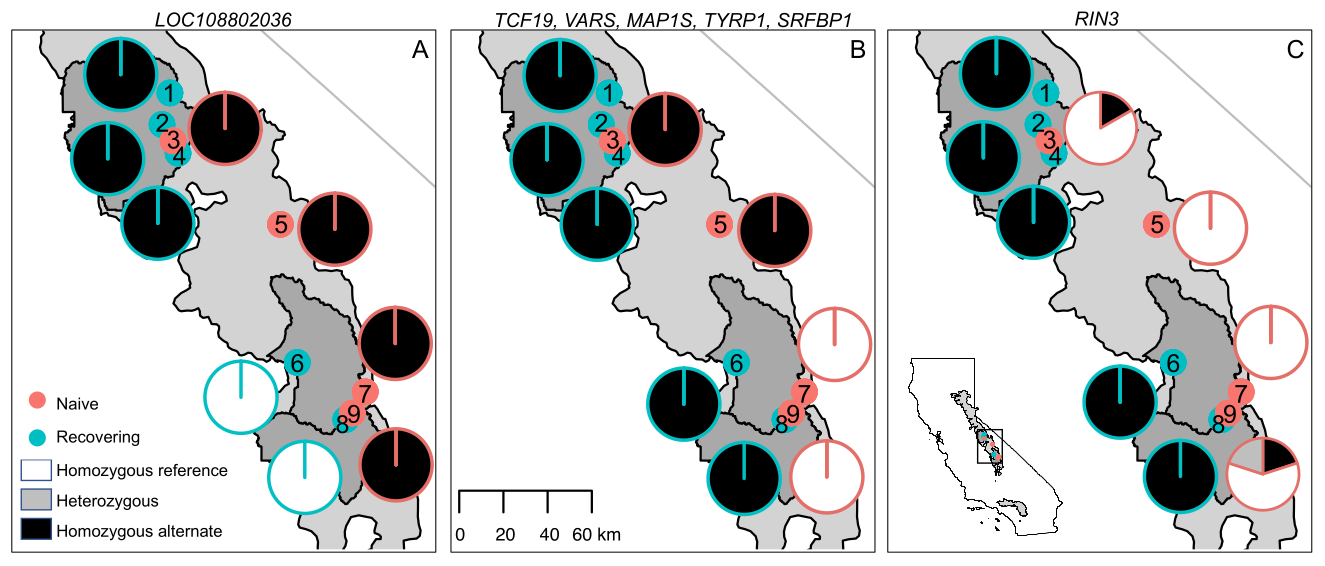
\includegraphics[width=0.8\textwidth]{figures/allele_maps.png}

}

\caption{\label{fig-allelefrequencies}For each of the naive and
recovering MYL frog populations, pie charts showing allele frequencies
for the 11 outlier SNPs from 7 distinct genes: (A) LOC108802036, (B)
TCF19, VARS, MAP1S, TYRP1, SRFBP1, and (C) RIN3. Charts are superimposed
on a map of the Sierra Nevada study area, with Yosemite, Kings Canyon,
and Sequoia National Parks (from north to south) shown in dark gray, and
the range boundary for MYL frogs in this portion of the Sierra Nevada
shown in light gray. The inset map locates the study area in
California.}

\end{figure*}

\newpage

\begin{figure*}

{\centering 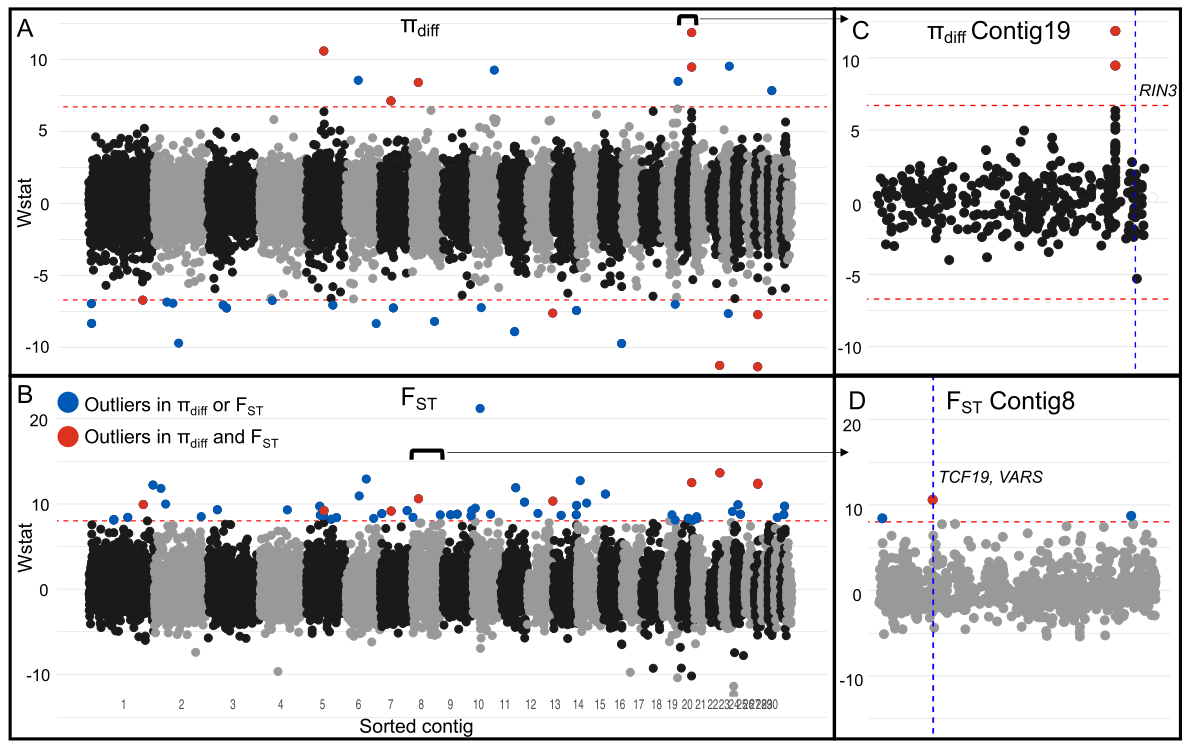
\includegraphics[width=0.8\textwidth]{figures/splinewindow_manhattan.png}

}

\caption{\label{fig-spline-manhattan}Results from the splined window
analysis showing outlier windows for the difference in nucleotide
diversity \(\pi_{diff}\) (A) and \emph{F\textsubscript{ST}} (B). Outlier
regions for either \(\pi_{diff}\) or \emph{F\textsubscript{ST}} are
shown in blue and outlier regions for both \(\pi_{diff}\) and
\emph{F\textsubscript{ST}} are shown in red. (C) Magnified Contig19 from
(A) showing two adjacent outlier windows for \(\pi_{diff}\) 12.9Mb
upstream of the RIN3 outlier SNP (indicated with a dashed vertical blue
line). (D) Magnified Contig8 from from (B) showing the
\emph{F\textsubscript{ST}} outlier window that includes the outlier SNPs
TCF19 and VARS. This region of the genome contains 8 annotated genes
known to occur in the extended MHC Class I and II regions.}

\end{figure*}

\newpage

\begin{figure*}

{\centering 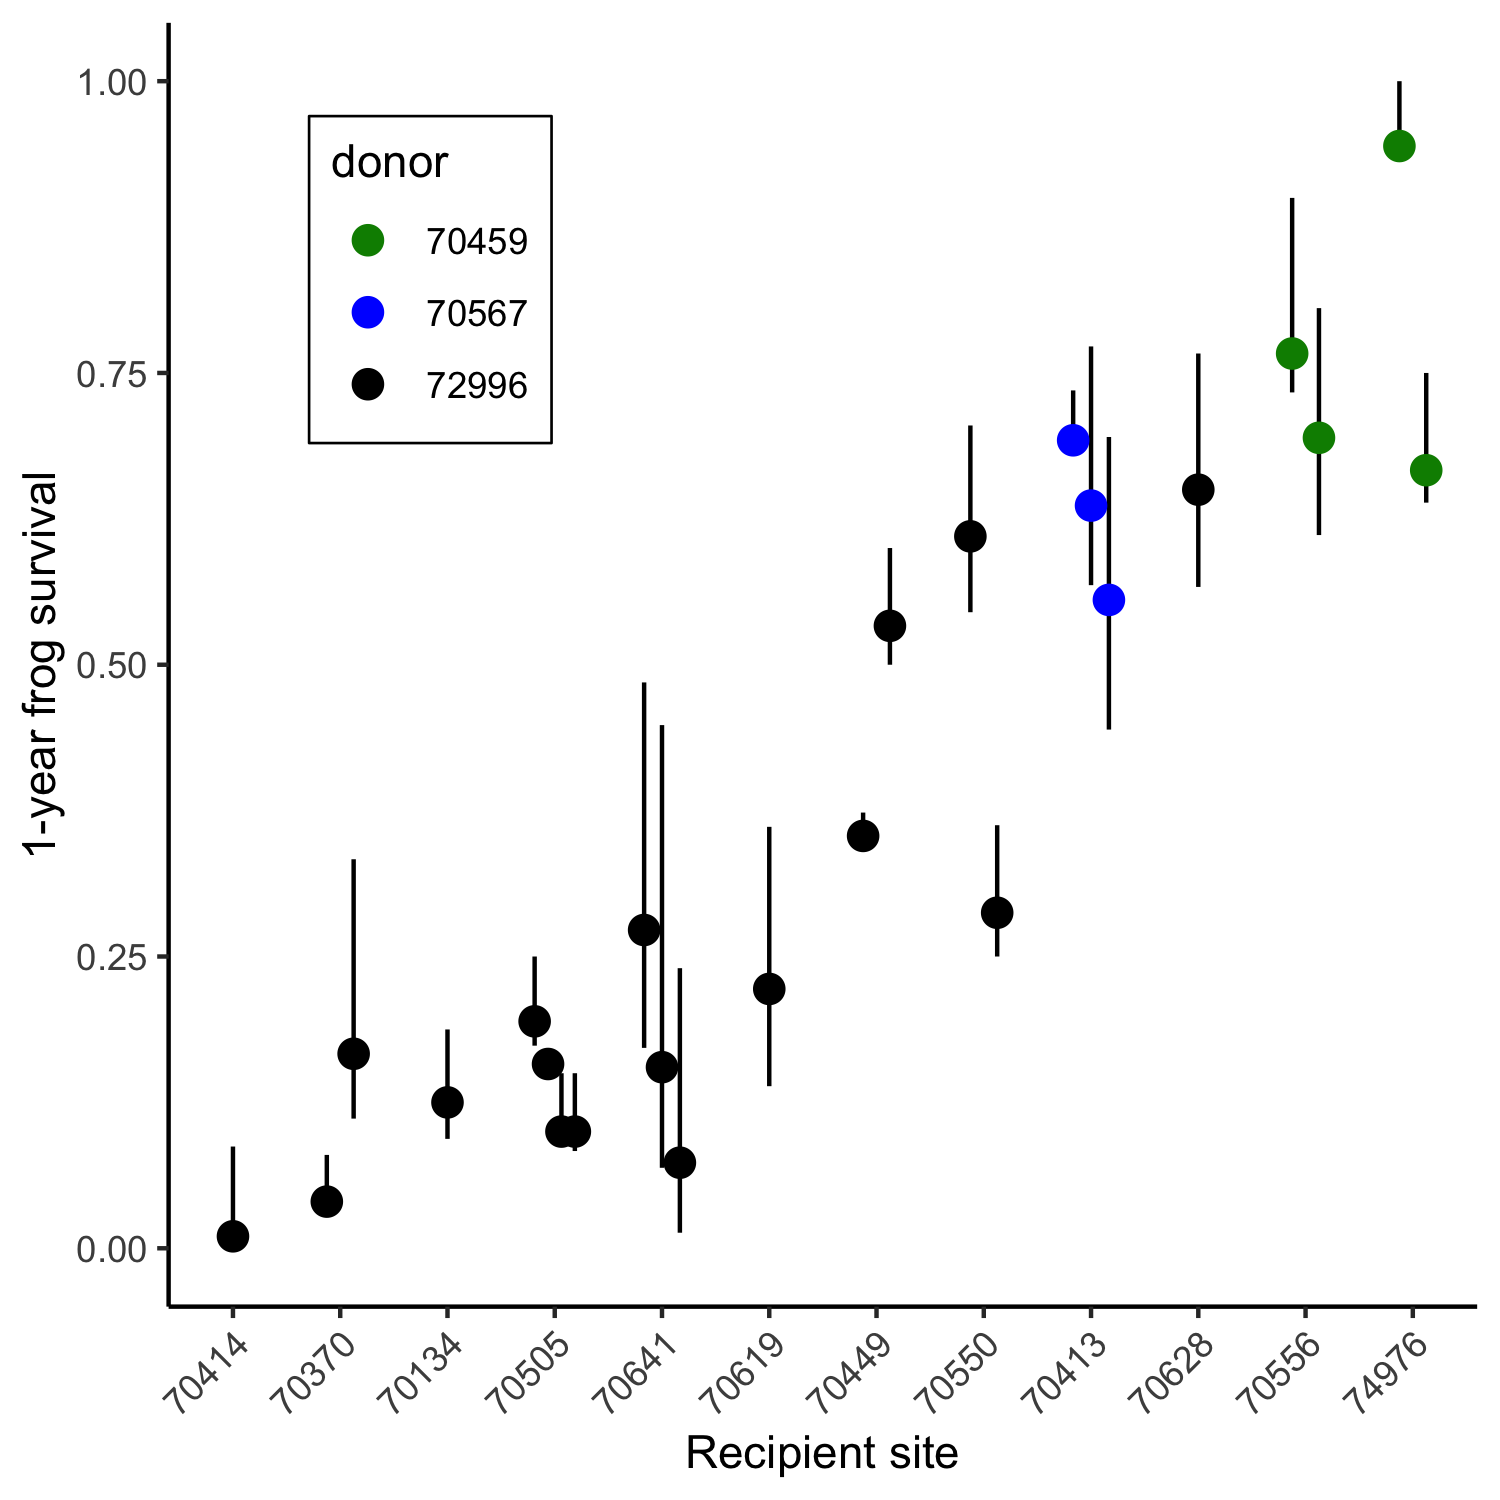
\includegraphics[width=0.8\textwidth]{figures/translocation_survival_bysiteid.png}

}

\caption{\label{fig-translocation-survival}Median 1-year survival for
each cohort of translocated frogs at the 12 recipient sites. Sites are
arranged along the x-axis using the average of the median 1-year
survival per translocation at each site. Dot colors indicate the donor
population from which frogs in each translocated cohort were collected.
Error bars show the 95\% uncertainty intervals. When multiple
translocations were conducted to a site, points and error bars are
slightly offset to avoid overlap.}

\end{figure*}

\newpage

\begin{figure*}

{\centering 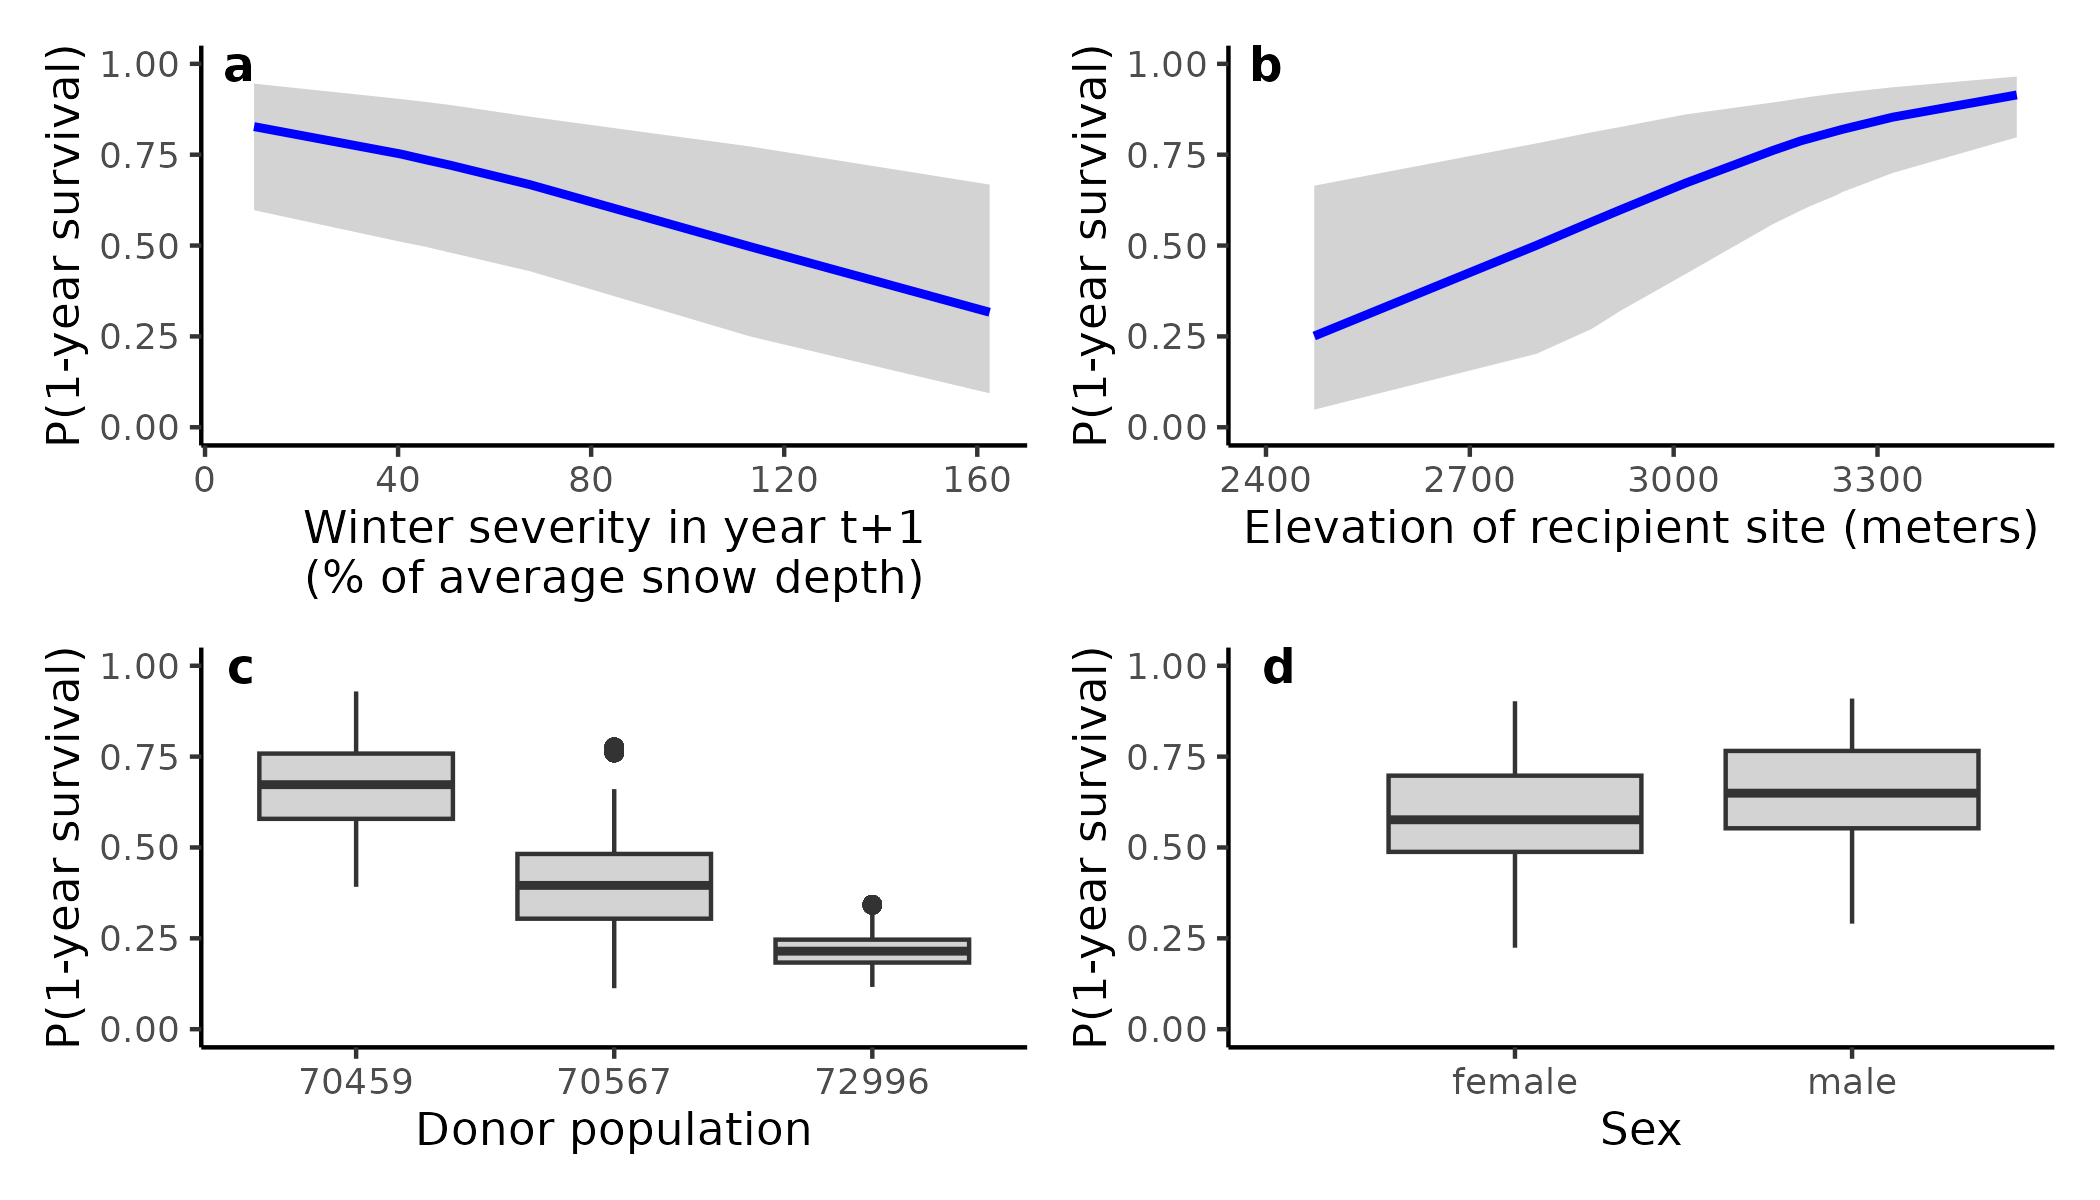
\includegraphics[width=0.8\textwidth]{figures/cond_effects_plot.png}

}

\caption{\label{fig-cond-effects}Results showing conditional effects of
the important predictors of 1-year frog survival. (A) winter severity in
the year following translocation, (B) elevation of recipient site, (C)
donor population, and (D) sex. In (A) and (B), blue lines are medians
and gray ribbons are 95\% uncertainty intervals. In (C) and (D), box
plots show medians, first and third quartiles, largest and smallest
values within 1.5x interquartile range, and values outside the 1.5x
interquartile range.}

\end{figure*}

\newpage

\begin{figure*}

{\centering 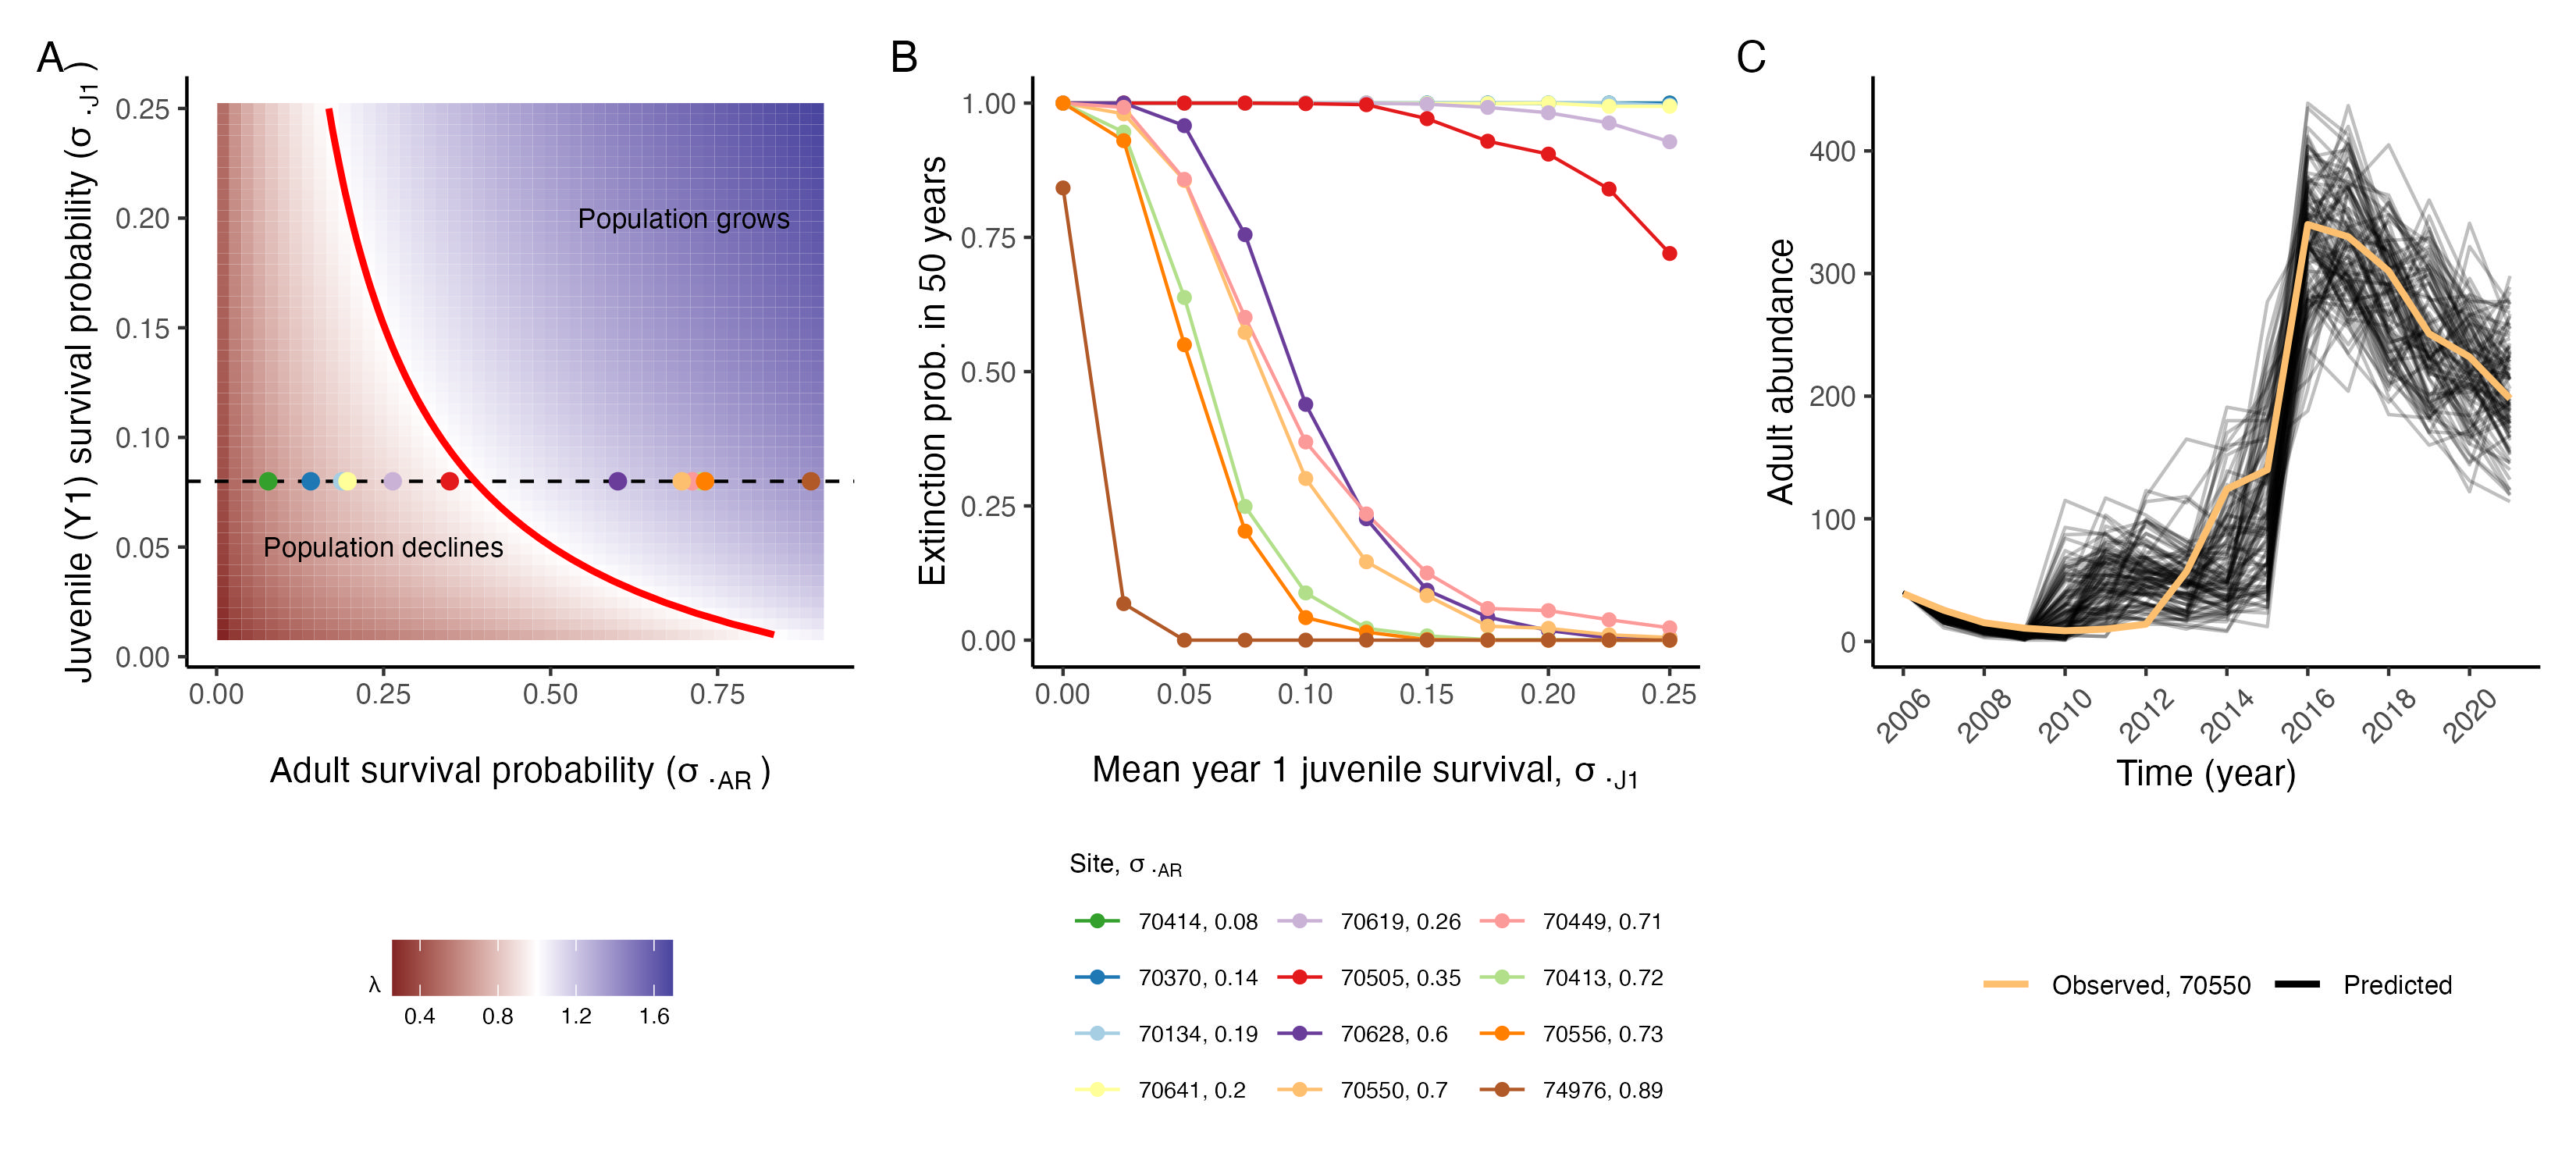
\includegraphics[width=0.8\textwidth]{figures/pop_viability_figures_for_manuscript.jpg}

}

\caption{\label{fig-viability}A population viability analysis of
translocated MYL frogs that quantifies the long-run growth rate and
extinction probability of frog populations: (A) Predicted long-run
growth rate \$\textbackslash lambda\$ for different values of yearly
adult survival probability \$\textbackslash sigma\_\{A\_R\}\$ and
probability of recruitment \$\textbackslash omega\$, given the
parameterized, deterministic model. Colored points show the predicted
\$\textbackslash lambda\$ values for the twelve translocated populations
when probability of recruitment into the adult class is
\$\textbackslash omega = 0.3\$ (indicated by the dashed line). The red
line shows where \$\textbackslash lambda = 1\$. (B) Predicted 50-year
extinction probabilities of the 12 translocated populations given
demographic stochasticity, environmental variability in
\$\textbackslash omega\$, and different mean values of
\$\textbackslash omega\$. The dashed line shows where
\$\textbackslash omega = 0.3\$, for comparison to (A). There are 6 lines
at extinction probability = 1, 5 of which (70414--70619) are hidden
beneath the line for 70505.}

\end{figure*}

\newpage

\begin{figure*}

{\centering 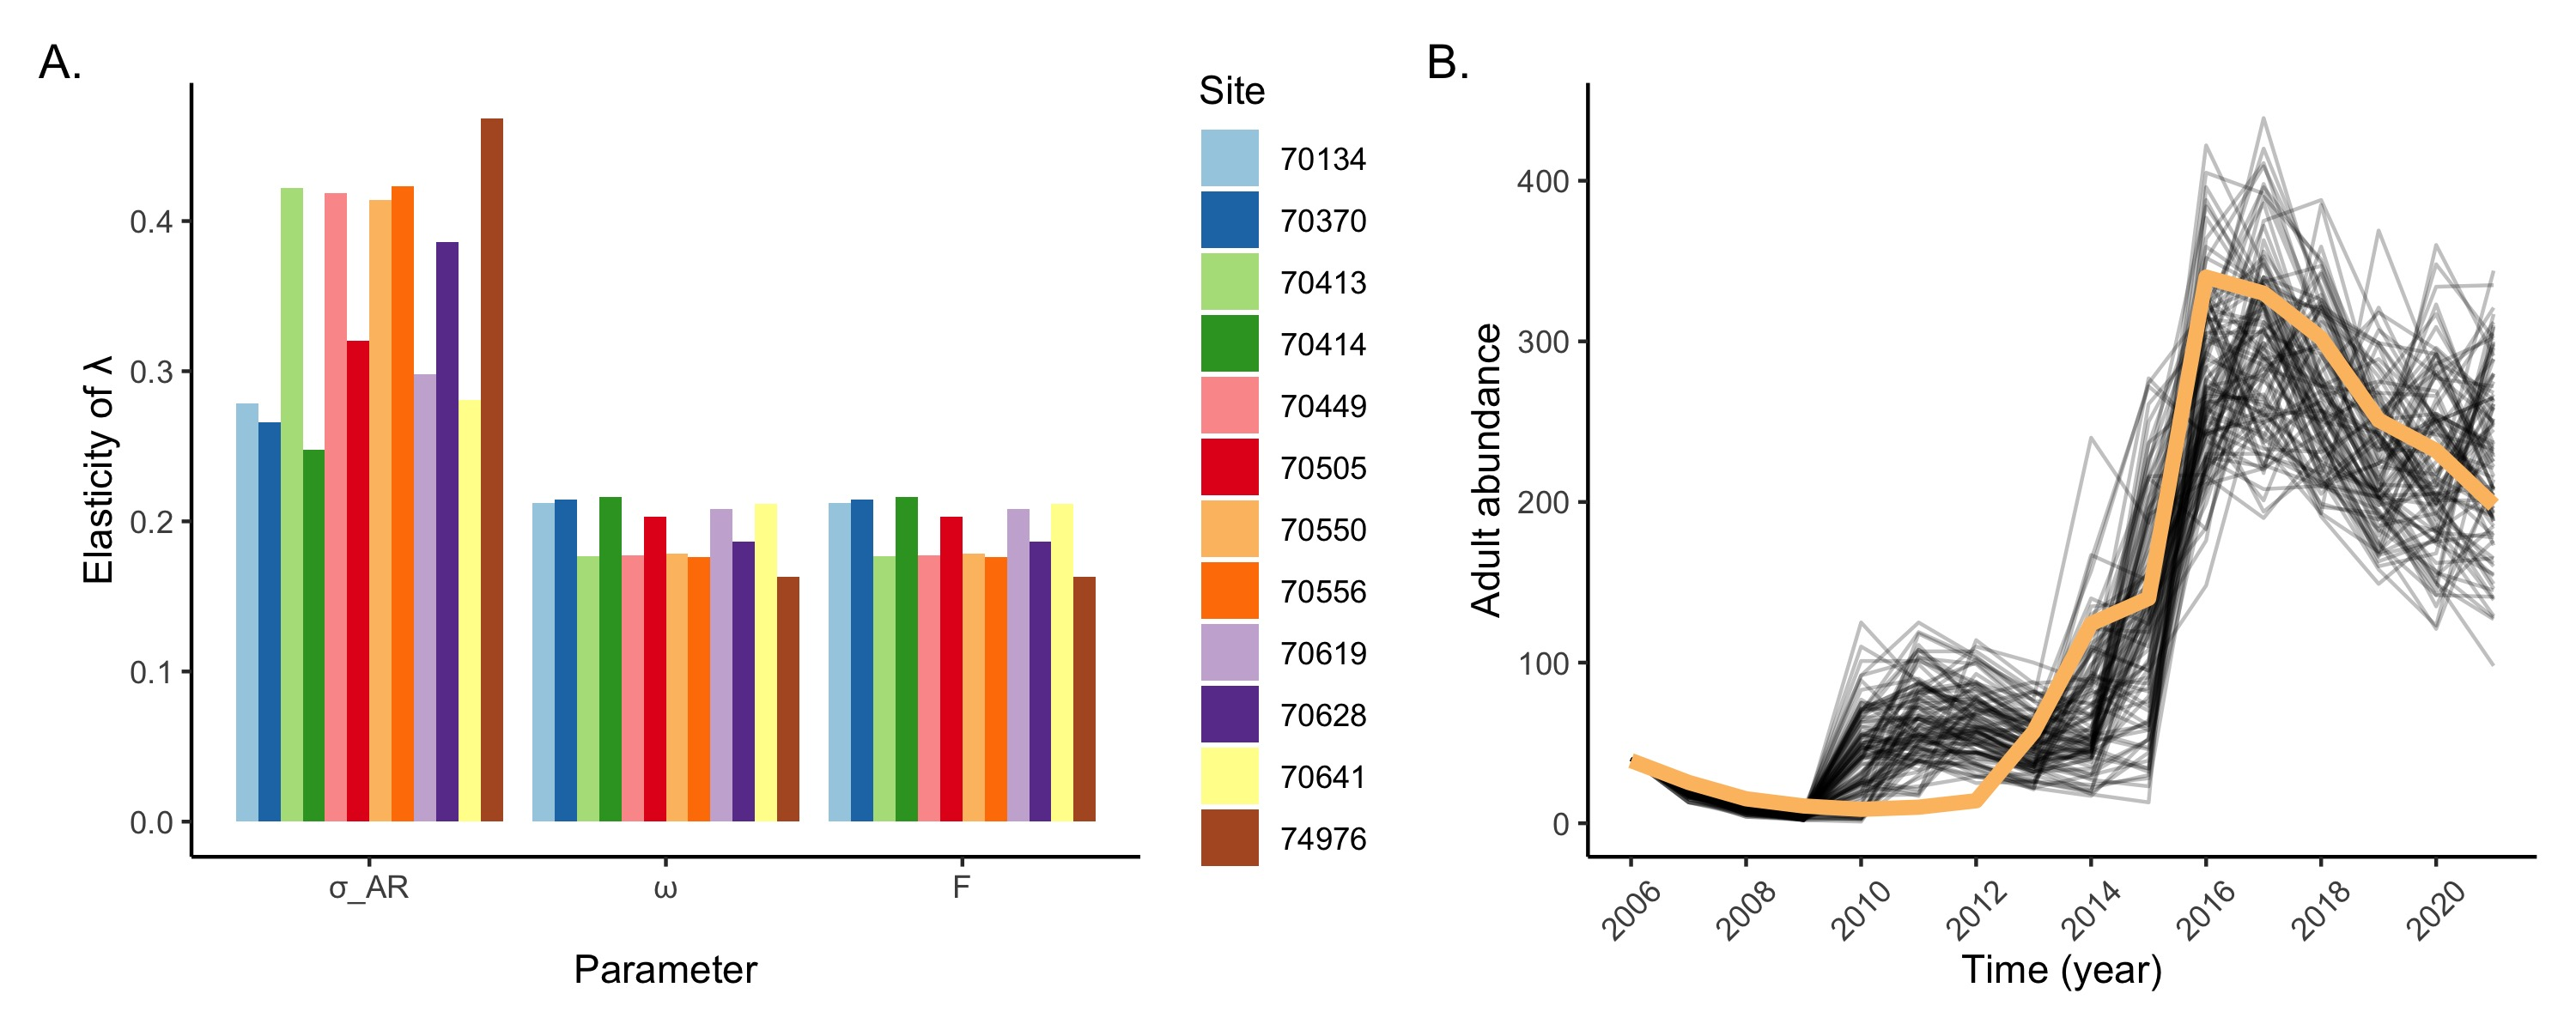
\includegraphics[width=0.8\textwidth]{figures/pop_viability_figures_for_supp.jpg}

}

\caption{\label{fig-viability-supp}Sensitivity analysis and empirical
validation of the stage-structured MYL frog model. (A) Elasticity of
\(\lambda\) with changes in 3 parameters: \(\sigma_{A_R}\) (yearly
survival probability of naturally recruited adults), \(\omega\) (yearly
probability of successful recruitment from juveniles to adults), and
\emph{F (}number of eggs produced by a female frog in a year that
successfully hatch). Elasticity is calculated at the default parameter
values for each population and \(\omega\) = 0.3. (B) 100 simulated
trajectories (black lines) that most closely matched the observed
abundance trajectory of adult amphibians at site 70550 (light orange).}

\end{figure*}

\newpage
\end{document}

